\newpage
\section{Inventory}
\label{sec:inventory}

\begin{figure}[ht]
	\centering
  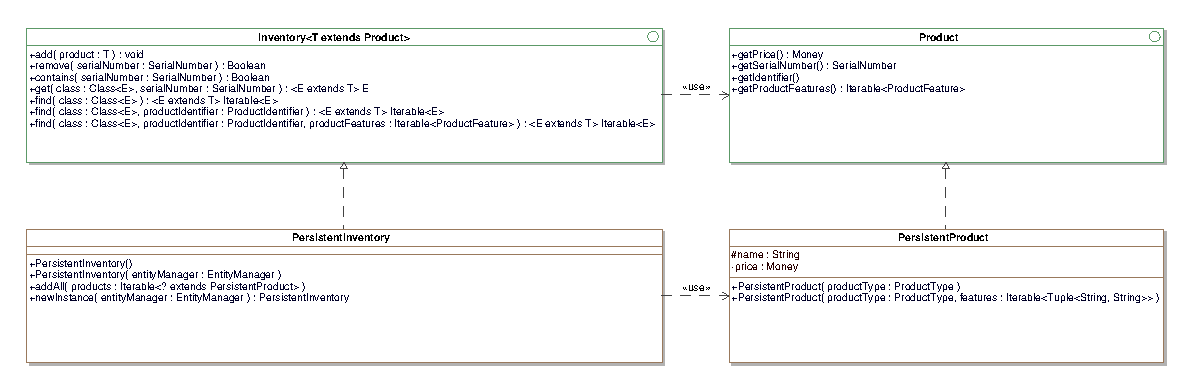
\includegraphics[width=1.0\textwidth]{images/Inventory_Overview.eps}
	\label{inventory_overview}
	\caption{Inventory - Class Overview}
\end{figure}

%\subsection{\code{Inventory} - Managing products} 

\code{Inventory} is an interface and provides methods for adding and removing products as well as finding products based on the \code{ProductType} via the \code{ProductTypeIdentifier} and a set of \code{ProductFeature}s.
\code{PersistentInventory} is an implementation of the \code{Inventory} interface. Every operation is delegated to the database, via \code{CriteriaQuery}s. Some methods require additional processing of query results with Java.
\code{Inventory} aggregates \code{Product}s, \code{PersistentInventory} aggregates \code{PersistentProduct}s 

%A shop must store products in an inventory, because the customer should get your good on order very quickly. If there are no amount of this product inside, it must be ordered by its producer.
%This procedure can be implemented by the \code{PersistentInventory}-class. This class is an implementation of the interface \code{Inventory}, to used its functionality and also 
%to persist the items of your inventory.\\
%With the methods of the \code{Inventory}-class you can add one or many \code{Products} to the inventory, you can remove a product from it or you can checked, whether a product exist in it.
%Also you can find \code{Products} with several options, if you know the \code{ProductIdentifier}, their \code{productFeatures} or the classes of them.
